%% IMPORTANT: The official thesis specifications are available at:
%%            http://libraries.mit.edu/archives/thesis-specs/
%%
%%            Please verify your thesis' formatting and copyright
%%            assignment before submission.  If you notice any
%%            discrepancies between these templates and the
%%            MIT Libraries' specs, please let us know
%%            by e-mailing thesis@mit.edu

%% The documentclass options along with the pagestyle can be used to generate
%% a technical report, a draft copy, or a regular thesis.  You may need to
%% re-specify the pagestyle after you \include  cover.tex.  For more
%% information, see the first few lines of mitthesis.cls.

%\documentclass[12pt,vi,twoside]{mitthesis}
%%
%%  If you want your thesis copyright to you instead of MIT, use the
%%  ``vi'' option, as above.
%%
%\documentclass[12pt,twoside,leftblank]{mitthesis}
%%
%% If you want blank pages before new chapters to be labelled ``This
%% Page Intentionally Left Blank'', use the ``leftblank'' option, as
%% above.

\documentclass[12pt,twoside]{mitthesis}
\usepackage{lgrind}
\pagestyle{plain}

%% This bit allows you to either specify only the files which you wish to
%% process, or `all' to process all files which you \include.
%% Krishna Sethuraman (1990).

% \typein [\files]{Enter file names to process, (chap1,chap2 ...), or `all' to
% process all files:}
% \def\all{all}
% \ifx\files\all \typeout{Including all files.} \else \typeout{Including only \files.} \includeonly{\files} \fi

\def\thetitle{Realization of Bose-Einstein Condensation with Lithium-$7$ Atoms}

\usepackage[pdftex,pdfauthor={Yichao Yu},pdftitle={\thetitle}]{hyperref}

\newcommand{\ud}{\mathrm{d}}
\newcommand{\ue}{\mathrm{e}}
\newcommand{\ui}{\mathrm{i}}
\newcommand{\res}{\mathrm{Res}}
\newcommand{\Tr}{\mathrm{Tr}}
\newcommand{\dsum}{\displaystyle\sum}
\newcommand{\dprod}{\displaystyle\prod}
\newcommand{\dlim}{\displaystyle\lim}
\newcommand{\dint}{\displaystyle\int}
\newcommand{\fsno}[1]{{\!\not\!{#1}}}
\newcommand{\eqar}[1]
{
  \begin{align*}
    #1
  \end{align*}
}
\newcommand{\texp}[2]{\ensuremath{{#1}\times10^{#2}}}
\newcommand{\dexp}[2]{\ensuremath{{#1}\cdot10^{#2}}}
\newcommand{\eval}[2]{{\left.{#1}\right|_{#2}}}
\newcommand{\paren}[1]{{\left({#1}\right)}}
\newcommand{\lparen}[1]{{\left({#1}\right.}}
\newcommand{\rparen}[1]{{\left.{#1}\right)}}
\newcommand{\abs}[1]{{\left|{#1}\right|}}
\newcommand{\sqr}[1]{{\left[{#1}\right]}}
\newcommand{\crly}[1]{{\left\{{#1}\right\}}}
\newcommand{\angl}[1]{{\left\langle{#1}\right\rangle}}
\newcommand{\tpdiff}[4][{}]{{\paren{\frac{\partial^{#1} {#2}}{\partial {#3}{}^{#1}}}_{#4}}}
\newcommand{\tpsdiff}[4][{}]{{\paren{\frac{\partial^{#1}}{\partial {#3}{}^{#1}}{#2}}_{#4}}}
\newcommand{\pdiff}[3][{}]{{\frac{\partial^{#1} {#2}}{\partial {#3}{}^{#1}}}}
\newcommand{\diff}[3][{}]{{\frac{\ud^{#1} {#2}}{\ud {#3}{}^{#1}}}}
\newcommand{\psdiff}[3][{}]{{\frac{\partial^{#1}}{\partial {#3}{}^{#1}} {#2}}}
\newcommand{\sdiff}[3][{}]{{\frac{\ud^{#1}}{\ud {#3}{}^{#1}} {#2}}}
\newcommand{\tpddiff}[4][{}]{{\left(\dfrac{\partial^{#1} {#2}}{\partial {#3}{}^{#1}}\right)_{#4}}}
\newcommand{\tpsddiff}[4][{}]{{\paren{\dfrac{\partial^{#1}}{\partial {#3}{}^{#1}}{#2}}_{#4}}}
\newcommand{\pddiff}[3][{}]{{\dfrac{\partial^{#1} {#2}}{\partial {#3}{}^{#1}}}}
\newcommand{\ddiff}[3][{}]{{\dfrac{\ud^{#1} {#2}}{\ud {#3}{}^{#1}}}}
\newcommand{\psddiff}[3][{}]{{\frac{\partial^{#1}}{\partial{}^{#1} {#3}} {#2}}}
\newcommand{\sddiff}[3][{}]{{\frac{\ud^{#1}}{\ud {#3}{}^{#1}} {#2}}}

\begin{document}

\include{cover}
% Some departments (e.g. 5) require an additional signature page.  See
% signature.tex for more information and uncomment the following line if
% applicable.
% \include{signature}
\pagestyle{plain}
\include{contents}
\chapter{Introduction}

Predicted in 1924-25 by Satyendra Nath Bose and Albert Einstein from Bose statistics, the Bose Einstein condensate is a phase of matter at ultra-cold temperature that emerges completely because of quantum effects. It was first produced in the laboratory in 1995-96 at the University of Colorado Boulder, Massachusetts Institute of Technology and Rice University using laser cooling and evaporative cooling techniques. Since then, people have been using it to study many quantum effects. Among them, one effort is to simulate complex condensed matter systems using simplfied and well controlled model systems created by loading BEC into optical lattices.\\
\\
In our experiment, we use the Lithium-$7$ atoms to create a Bose-Einstein condensate. Because of the lightness and several Feshbach resonances, the Lithium-$7$ atom has very fast dynamics and great tunability, making it a perfect candidate for simulating and studying the phase diagrams of certain condensed matter models. The ultimate goal of the experiment is to study the anti-ferromagnetic phase in the anisotropic Heisenberg model ($XXZ$ model), and the work in this thesis focuses on getting a Bose-Einstein condensate using Lithium-$7$, which is one of the important steps before studying the system in an optical lattice.\\
\\
The presentation of this thesis is divided into two chapters. In the first chapter, I discuss the theory of our experiment, including the Bose-Einstein condensate (BEC) and the various cooling and trapping techniques we use. The second chapter describes the setup of the experiment, the alignment and optimization procedure we developed and the experimental results we have got for each steps.

\chapter{Theory}

\section{Theory of Degenerate Bose Gas}\label{ch1:bec}
\subsection{Bose-Einstein Condensate in Harmonic Trap}
\subsection{Effect of interaction}

\section{Laser Lock}

\section{Zeeman Slower}

\section{Magneto-Optical Trap}

\section{Gray Molasses}

\section{Evaporation in Static Magnetic Trap}

\section{Evaporation in Optical Dipole Trap}

\chapter{Experimental Setup and Results}

In this chapter, I will describe our experimental setup and results. It includes a breif discussion of our optical tables setup (\ref{exp:laser-table} and \ref{exp:machine-table}), the implementation, optimization and performance of each steps (\ref{exp:zeeman}, \ref{exp:mot}, \ref{exp:gm}, \ref{exp:pump}, \ref{exp:mt} and \ref{exp:odt}) and finally some basic characteristic of our BEC (\ref{exp:bec}).

\section{Laser System}\label{exp:laser-table}
The laser table is where we prepare all the light resonance with the Lithium-$7$ transition ($\approx671nm$). As discussed in the previous chapter, there are four distinct lines that we need in the experiment, the combination of $D1$, $D2$ with $F1$, $F2$. At a certain time, we need either $D1$ or $D2$ light with the probability of using both $F1$ and $F2$ at the same time and the laser table is designed to do just this.\\
\begin{figure}
  \begin{center}
    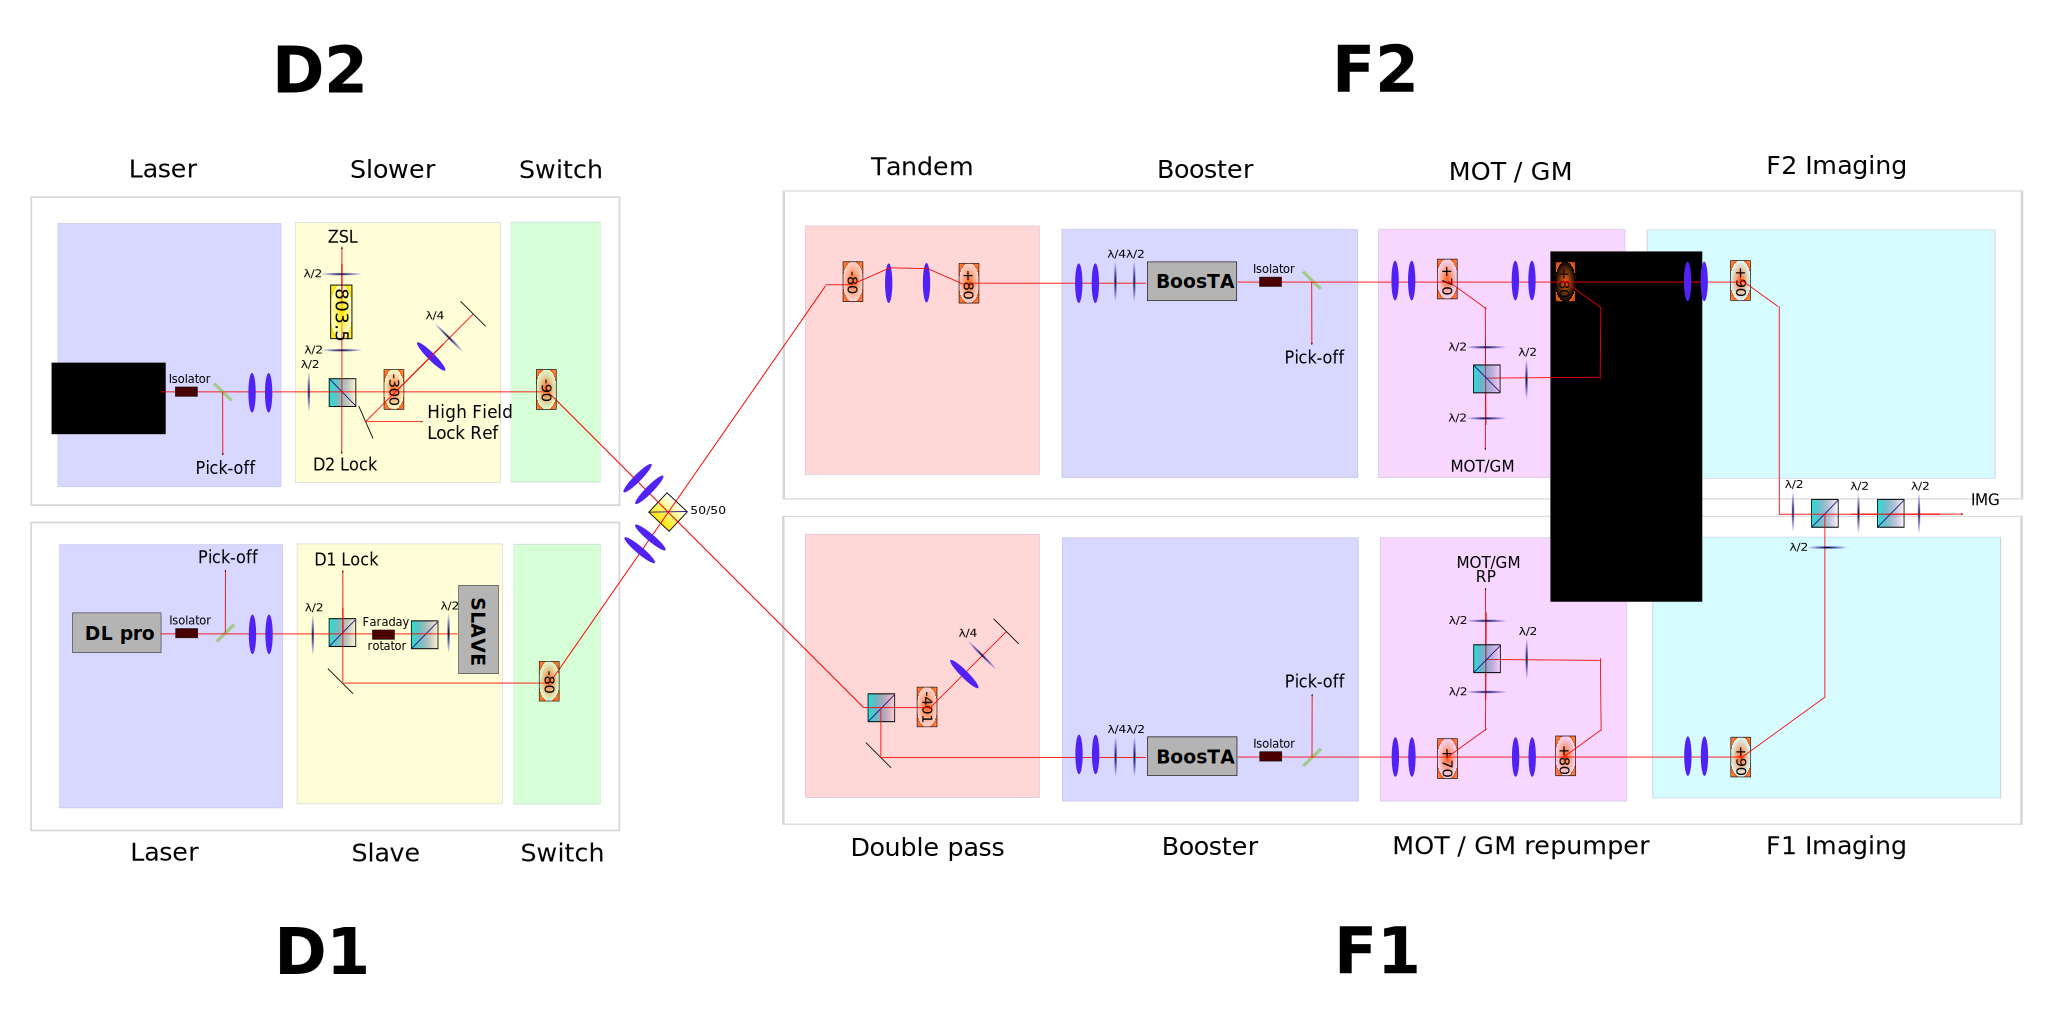
\includegraphics[width=14cm]{laser_table.png}
  \end{center}
  \caption{Schematic of the laser table design}
  \label{exp:laser-table-design}
\end{figure}\\
As shown in figure \ref{exp:laser-table-design}, since the separation between the $D1$ and $D2$ line ($\approx10GHz$) is larger than the range of common optical frequency shifters (e.g. AOM's), the $D1$ and $D2$ light are created separately using two diode lasers (TA pro and DL pro in figure \ref{exp:laser-table-design}). Both of these lasers are actively locked to the appropriate atomic transitions using saturated absorption spectroscopy to better than $2\text{MHz}$. For the $D2$ path, part of the light ($\approx80mW$) is red shifted and used as the Zeeman slower light ($ZSL$ in the figure) and the rest goes to the $D2$, $D1$ selecting switch, which uses two AOMs (acousto-optical modulator) and a $50$-$50$ cube to feed both the $F1$ and $F2$ path with either $D1$ and $D2$ light. For the $D1$ path, a slave diode is used to amplify the light before going to the switch.\\
\\
In the $F1$, $F2$ path, a tandem and a double pass are used to continiously shift the frequency of the laser (the double pass is also used to shift the light from $F2$ to $F1$). After that, the light in each path is amplified using tapered amplifier and then go through a polarization switch consists of two AOMs and a polarization beam splitter which can but the light into polarization maintaining fibers (MOT/GM and MOT/GM RP) with two orthogonal linear polarizations (the use of these beams is further described in section \ref{exp:mot-cage}). At the end of the chain, two more AOMs are used to control the light we put into the imaging fiber so that we can image on any of the four transitions. Each fibers also has a mechanical shutter that se used to block any possible leaking light that may cause heating.

\section{Vacuum Chamber and Main Coils Configuration}\label{exp:machine-table}

\subsection{MOT-Gray Molasses Cage}\label{exp:mot-cage}

\section{Spin Flip Zeeman Slower}\label{exp:zeeman}

\section{Magneto-Optical Trap (MOT) and Compressed-MOT}\label{exp:mot}

CMOT

\section{Gray Molasses}\label{exp:gm}

\section{Dark State Pumping}\label{exp:pump}

At the end of Laser cooling, the atoms are distributed in different ground states.\\
In order to trap in MT, need to go to 2, 2 / 2, 1 which are the only trappable states at both low field and high field.\\
Choose 2, 2 because we can use dark state pumping which ...

Dark State pumping with D1 light

Re-scattering, detuning

\section{Static Magnetic Trap}\label{exp:mt}

\section{Optical Dipole Trap}\label{exp:odt}

\section{Bose-Einstein Condensate}\label{exp:bec}

\appendix
% \include{appa}
% \include{appb}
\include{biblio}
\end{document}
